\section{解题流程图（补充说明）}

下面几张流程图是\key{补充材料}，供做题时对照使用，不单独作为知识点讲授。

\subsection{解一元二次不等式}

\begin{figure}[htbp]
  \centering
  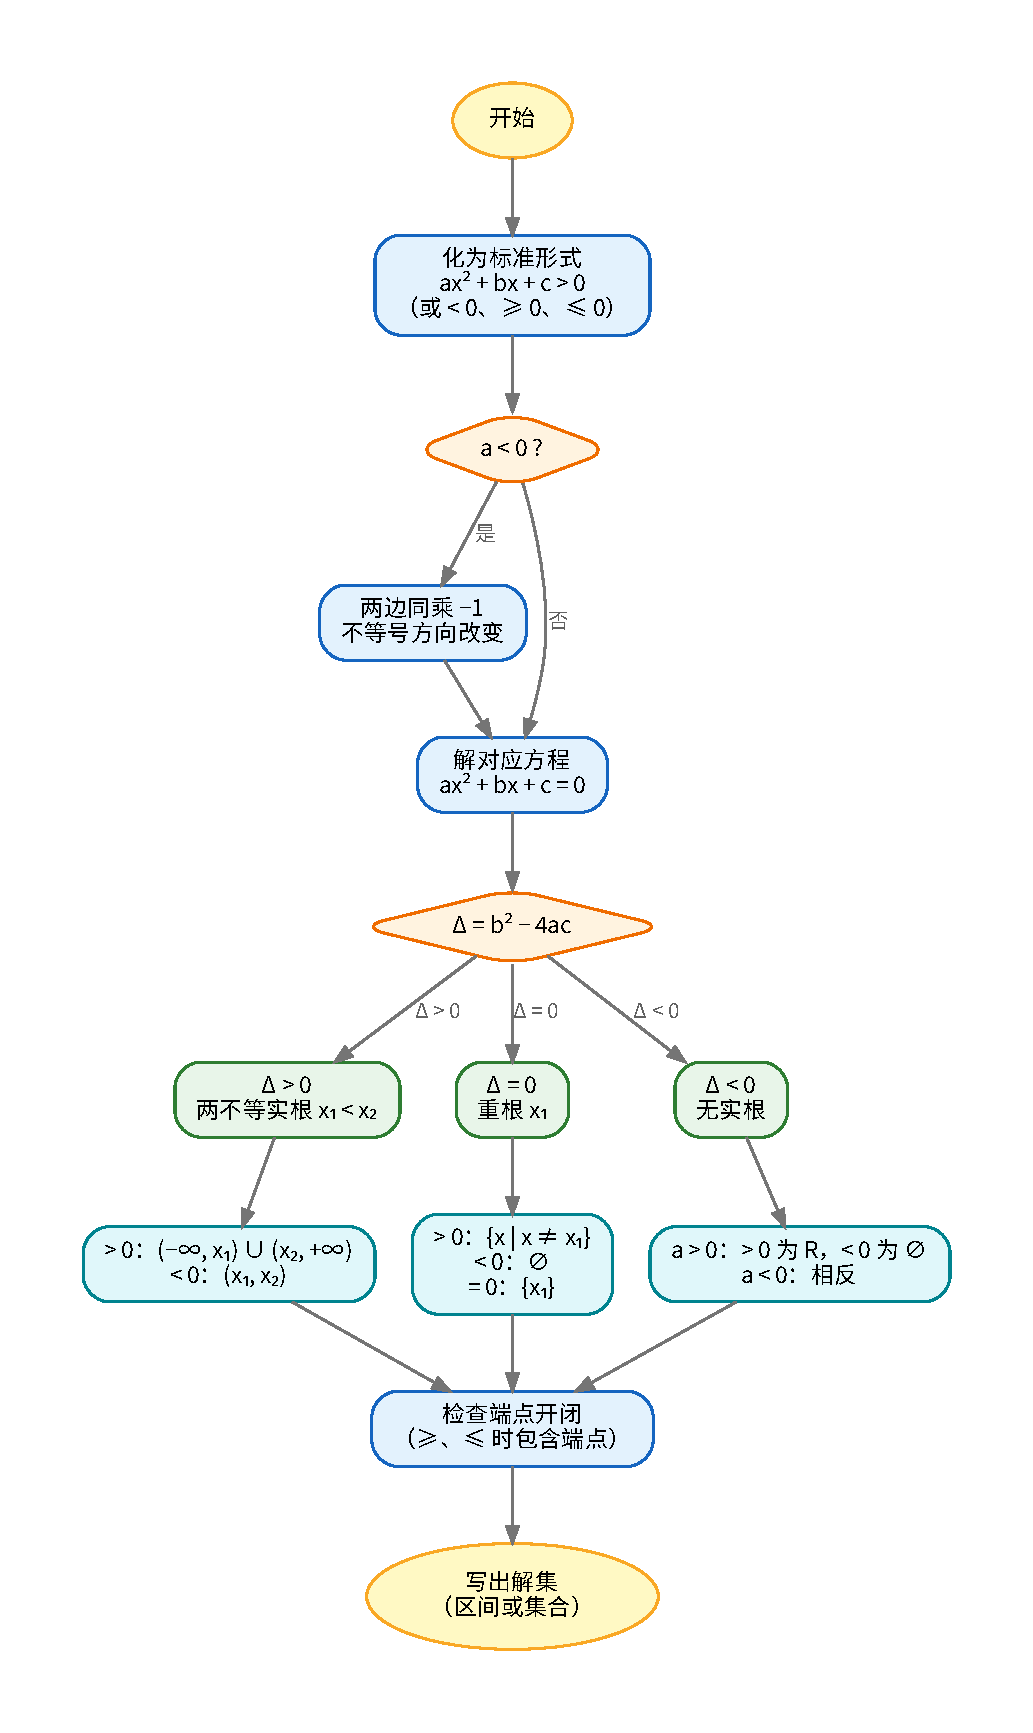
\includegraphics[width=0.60\textwidth]{flow-inequality.pdf}
  \caption{解一元二次不等式的完整流程}
\end{figure}

\key{一句话记忆}：先化正，再求根，后定区间，最后查端点。

\subsection{判断充分条件与必要条件}

\begin{figure}[htbp]
  \centering
  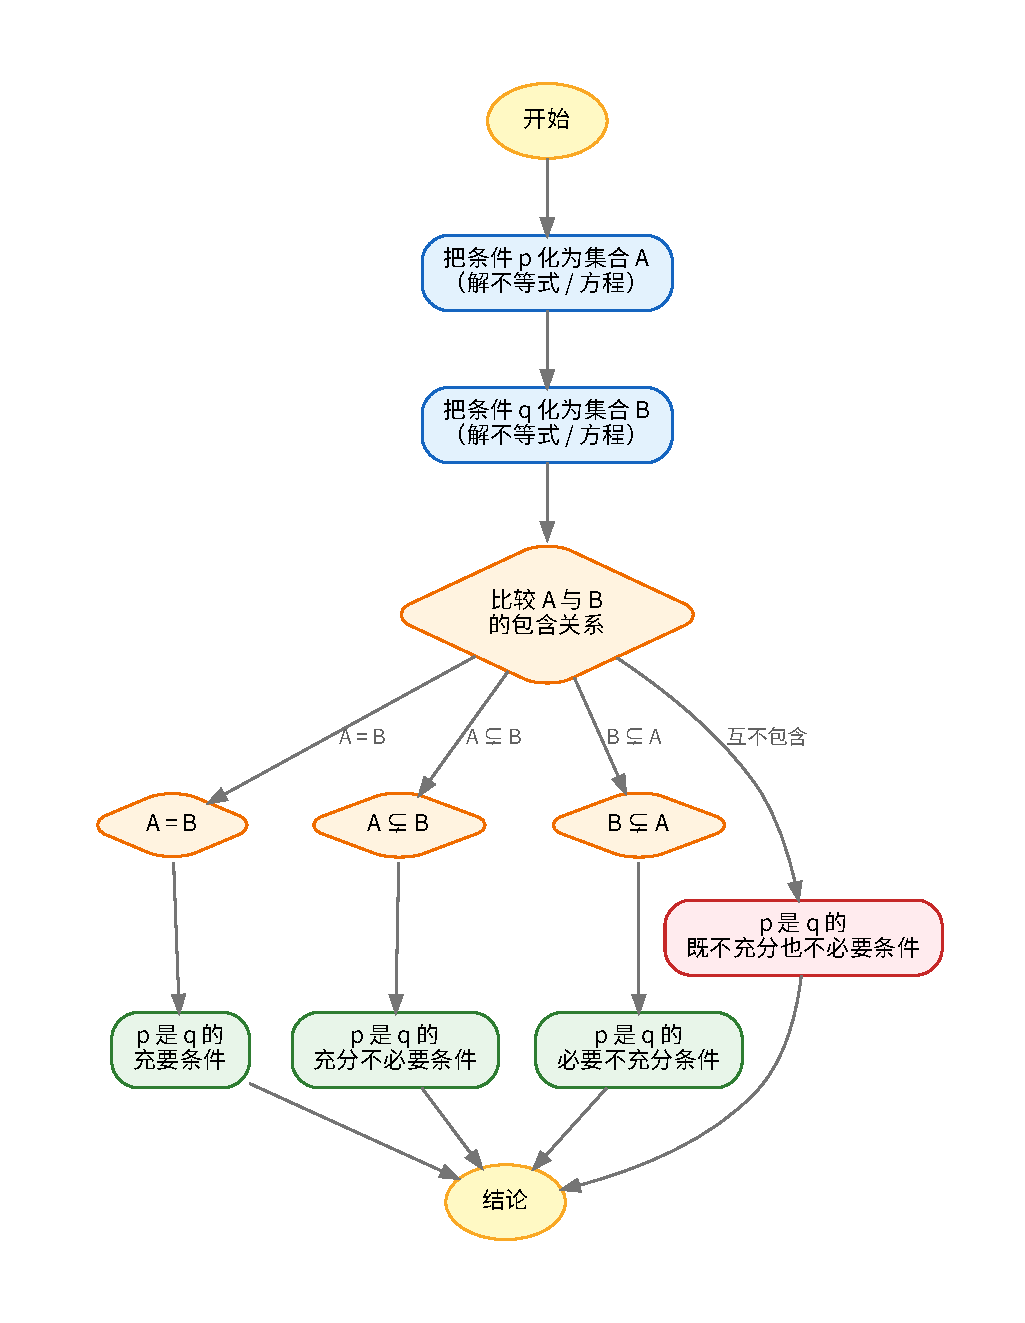
\includegraphics[width=0.60\textwidth]{flow-condition.pdf}
  \caption{用集合包含关系判断充分必要条件}
\end{figure}

\key{一句话记忆}：小范围推大范围，范围相等即充要。

\subsection{求二次函数在区间上的最值}

\begin{figure}[htbp]
  \centering
  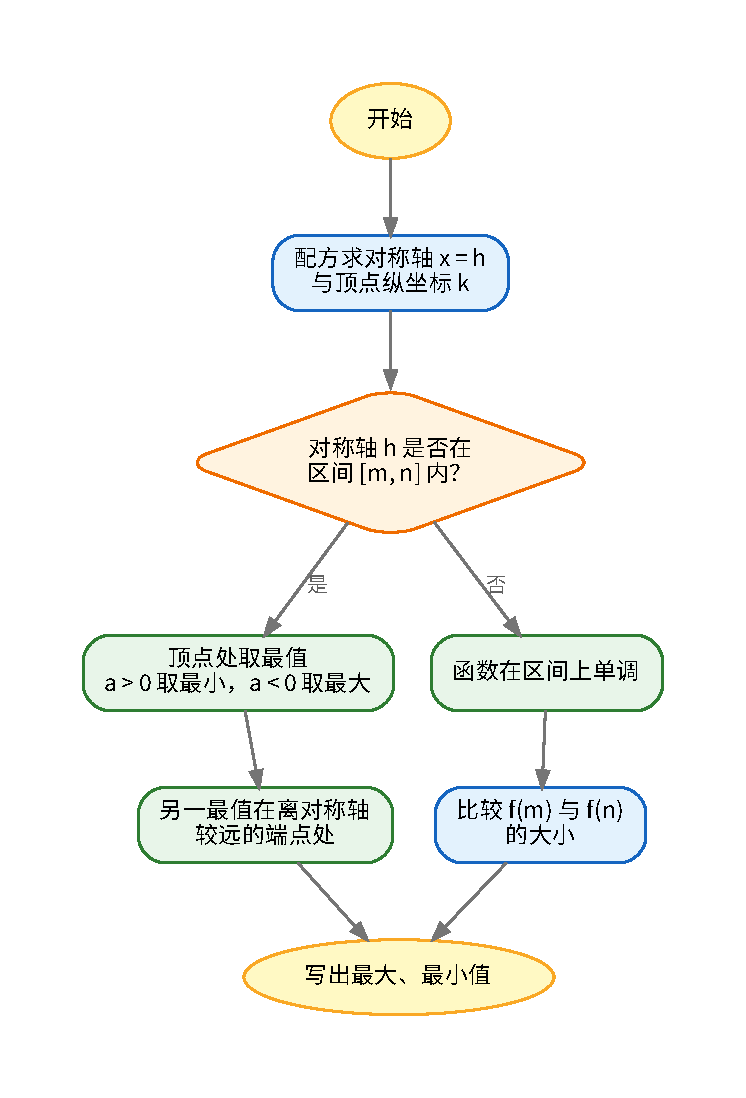
\includegraphics[width=0.60\textwidth]{flow-extreme.pdf}
  \caption{区间最值的分类讨论流程}
\end{figure}

\key{一句话记忆}：先看对称轴在不在区间内，在则顶点，不在则端点。

\subsection{解指数、对数不等式}

\begin{figure}[htbp]
  \centering
  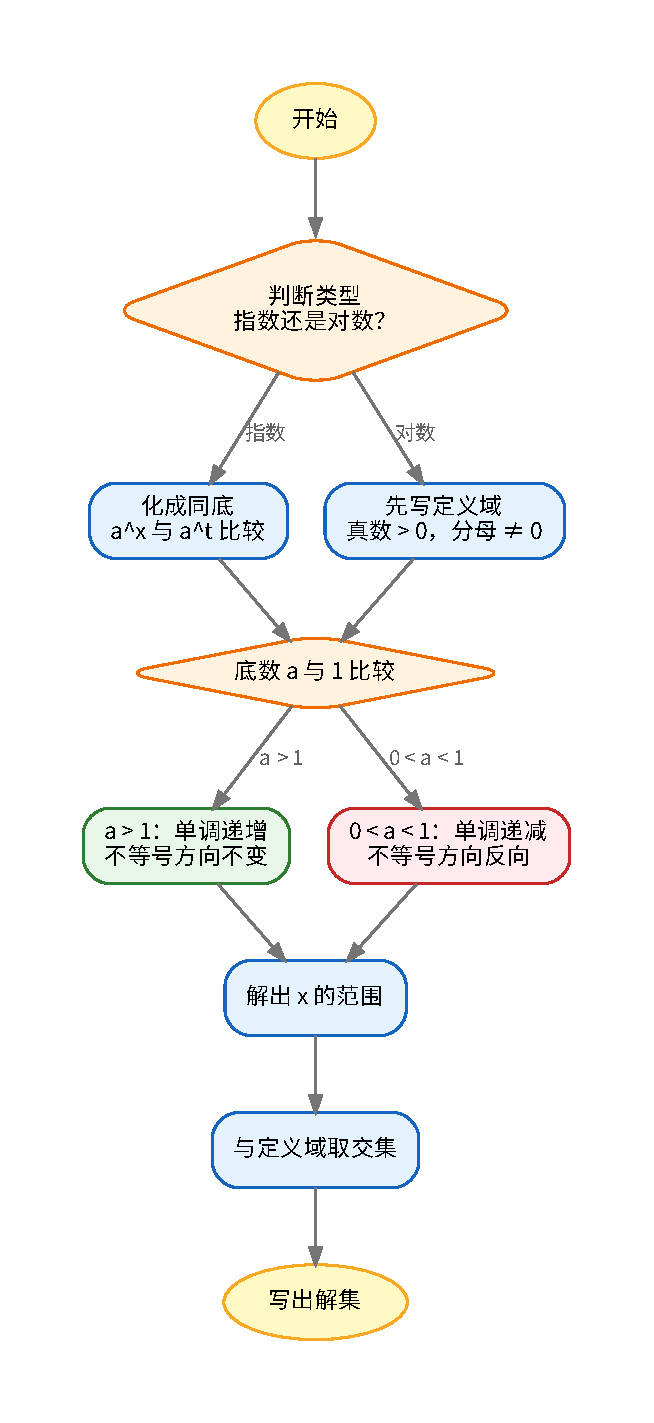
\includegraphics[width=0.62\textwidth]{flow-exp-log.pdf}
  \caption{解指数与对数不等式的流程}
\end{figure}

\key{一句话记忆}：先化同底，再看底数与 $1$ 的大小；对数别忘定义域。

\subsection{求 $y=A\sin(\omega x+\varphi)+b$ 的性质}

\begin{figure}[htbp]
  \centering
  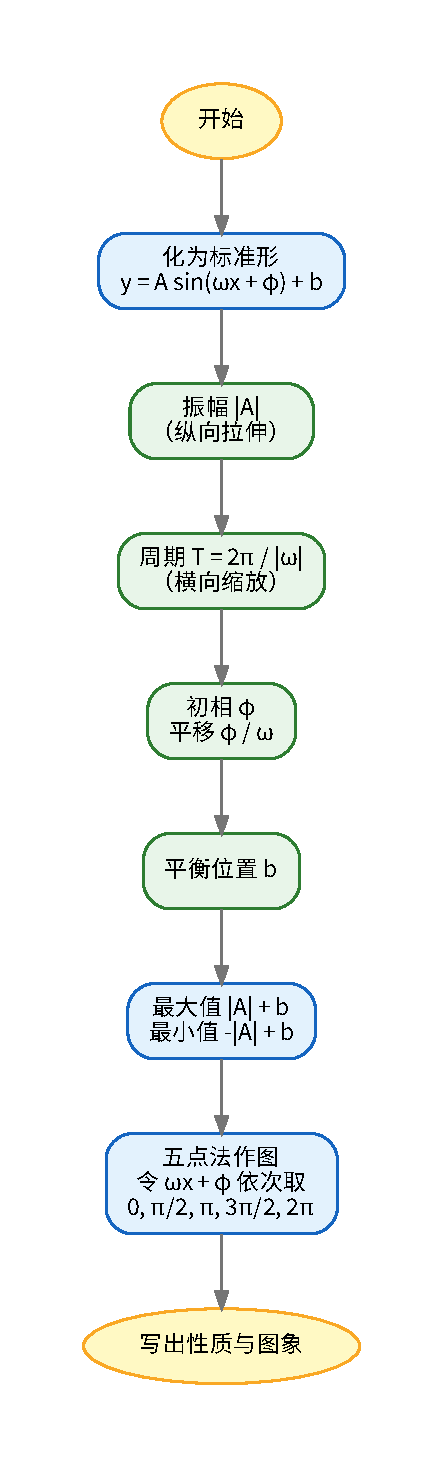
\includegraphics[width=0.56\textwidth]{flow-trig.pdf}
  \caption{由三个参数到图象与性质的流程}
\end{figure}

\key{一句话记忆}：$A$ 管高低，$\omega$ 管快慢，$\varphi$ 管左右，$b$ 管上下平移。

\subsection{流程图的用法}

流程图不是用来看的，是用来\key{照着做}的。建议：

\begin{enumerate}
  \item 做题时把流程图放在手边，一步一步对照；
  \item 每做一步，在题目上标出对应的是流程图中的哪一步；
  \item 做完十道题以后，尝试不对照流程图独立完成；
  \item 期末复习时，把流程图默写一遍。
\end{enumerate}
